\documentclass[tikz,border=10pt]{standalone}
\usetikzlibrary{shapes,arrows.meta,positioning}

\begin{document}
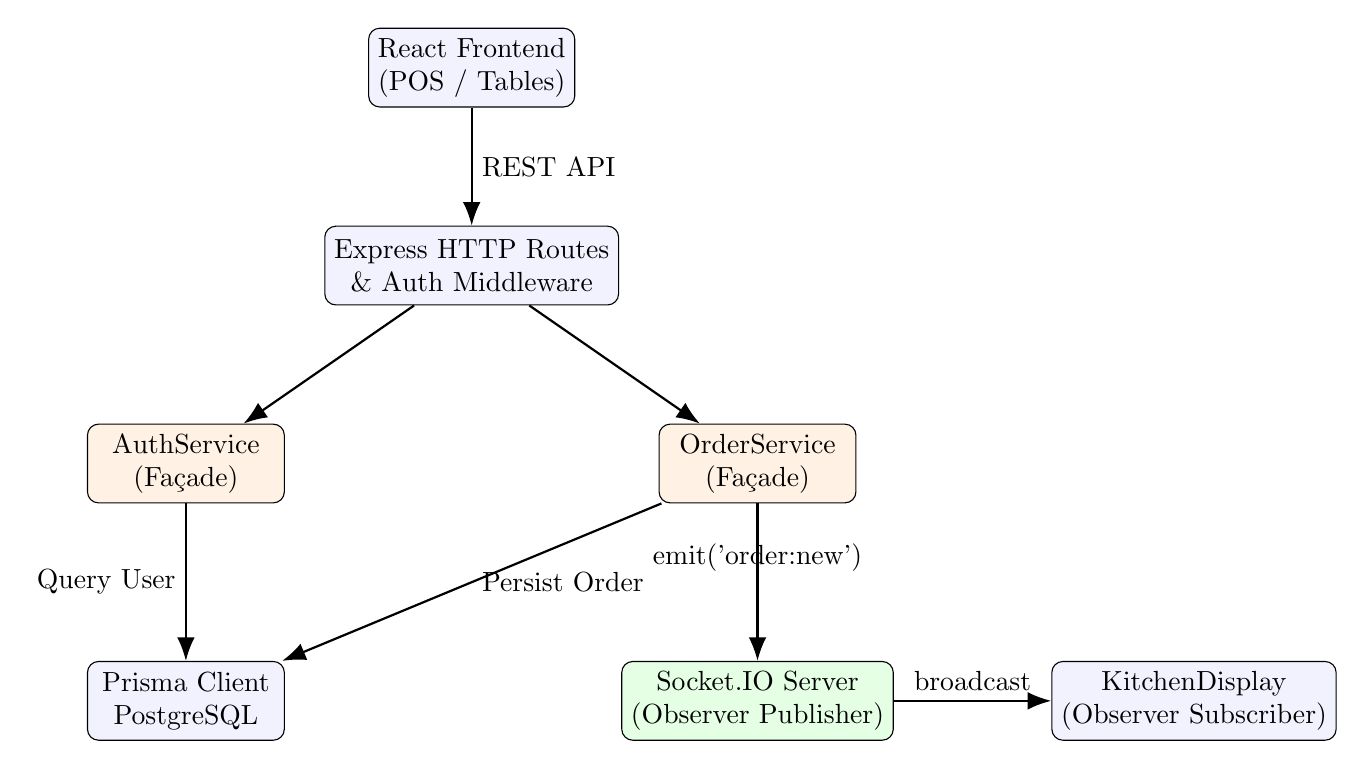
\begin{tikzpicture}[
    box/.style={draw, rectangle, rounded corners, minimum width=2.5cm, minimum height=1cm, align=center, fill=blue!5},
    facade/.style={draw, rectangle, rounded corners, minimum width=2.5cm, minimum height=1cm, align=center, fill=orange!10},
    obs/.style={draw, rectangle, rounded corners, minimum width=2.5cm, minimum height=1cm, align=center, fill=green!10},
    arrow/.style={-{Latex[length=3mm]}, thick}
]

\node[box] (react) {React Frontend\\(POS / Tables)};
\node[box, below=1.5cm of react] (routes) {Express HTTP Routes\\\& Auth Middleware};
\node[facade, below left=1.5cm and 0.5cm of routes] (authFacade) {AuthService\\(Fa\c{c}ade)};
\node[facade, below right=1.5cm and 0.5cm of routes] (orderFacade) {OrderService\\(Fa\c{c}ade)};
\node[box, below=2cm of authFacade] (prisma) {Prisma Client\\PostgreSQL};
\node[obs, below=2cm of orderFacade] (socket) {Socket.IO Server\\(Observer Publisher)};
\node[box, right=2cm of socket] (kitchen) {KitchenDisplay\\(Observer Subscriber)};

\draw[arrow] (react) -- node[right] {REST API} (routes);
\draw[arrow] (routes) -- (authFacade);
\draw[arrow] (routes) -- (orderFacade);
\draw[arrow] (authFacade) -- node[left] {Query User} (prisma);
\draw[arrow] (orderFacade) -- node[right] {Persist Order} (prisma);
\draw[arrow] (orderFacade) -- node[above] {emit('order:new')} (socket);
\draw[arrow] (socket) -- node[above] {broadcast} (kitchen);

\end{tikzpicture}
\end{document}
